\section{Konfiguration}
    \label{Konfiguration}

    Folgenden Abbildung zeigt das Konfigurationsmenü und seine Unterpunkte.
    \begin{figure}[H]
        \centering
        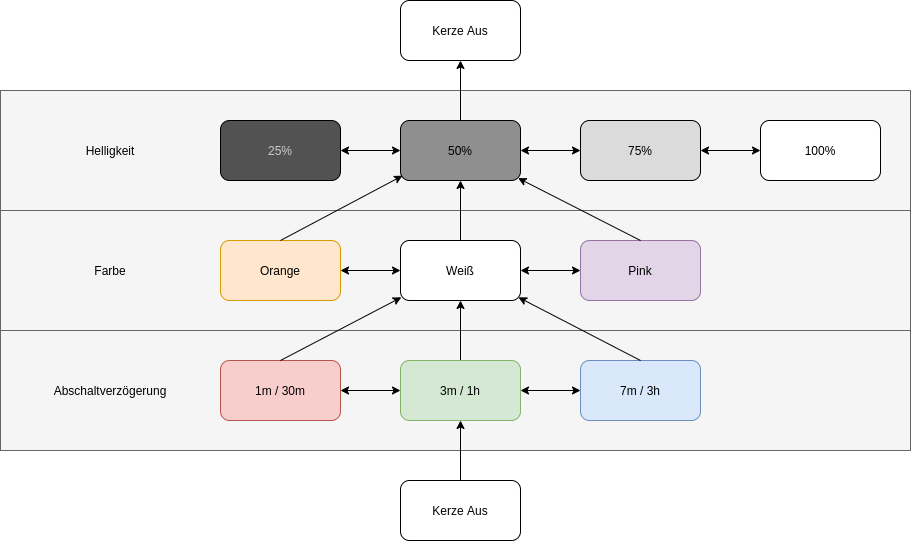
\includegraphics[scale=0.5]{img/Setup.png}
        \caption{Konfigurationsmenü}
    \end{figure}

    \subsection{Abschaltverzögerung}
        Die Abschaltverzögerung ist der erste Konfigurationsschritt und stellt
        drei Verzögerung zur Auswahl.
        Dabei wird zwischen den Abschaltverzögerung für den Laternenmodus und 
        dem Dekorationsmodus unterschieden. Wird zum Beispiel \textit{Rot} gewählt,
        schaltet sich die Kerze im Laternenmodus nach einer Minute und im
        Dekorationsmodus nach 30 Minuten ab. Dabei ist \textit{Rot} die
        Standardabschaltverzögerung nachdem die Kerze gestartet wurde.

        \begin{center}
            \begin{tabular}{| l | c | c |}
                \hline
                Farbe & Laternenmodus & Dekorationsmodus \\
                \hline
                Rot & 1m & 30m \\
                \hline
                Grün & 3m & 1h \\
                \hline
                Blau & 7m & 3h \\
                \hline
            \end{tabular}
        \end{center}


    \subsection{Farbe}
        Das Einstellen der Kerzenfarbe, ist der zweite Konfigurationsschritt
        und stellt Weiß, Orange und Pink zur Auswahl.
        Orange ist die Standardfarbe nachdem die Kerze gestartet wurde.

    \subsection{Helligkeit}
        Das Einstellen der kerzen Helligkeit ist der dritte und letzte Konfigurationsschritt.
        Dabei werden Helligkeiten von 25\%, 50\%, 75\% und 100\% zur Auswahl gestellt.
        50\% ist die Standardhelligkeit nachdem die Kerze gestartet wurde.

    \subsection{Zurücksetzen}
        Um alle Werte wieder auf Werkszustand zurück zu setzen, wird die Kerze 
        für einen kurzen Moment stromlos geschaltet. Nach dem Wiedereinsetzen
        des Akkus sind die Werte zurückgesetzt.
        